\section{Mission and Objectives}
\label{sec:Introduction}

Intro (date, time, and information of general flight.  Weather conditions.  Official flight time.  Float start time and date, along with termination time and date.  Impact location.  Did it all go well?

\begin{figure}[h!]
  \begin{center}
    \begin{minipage}[c]{0.45\linewidth}
      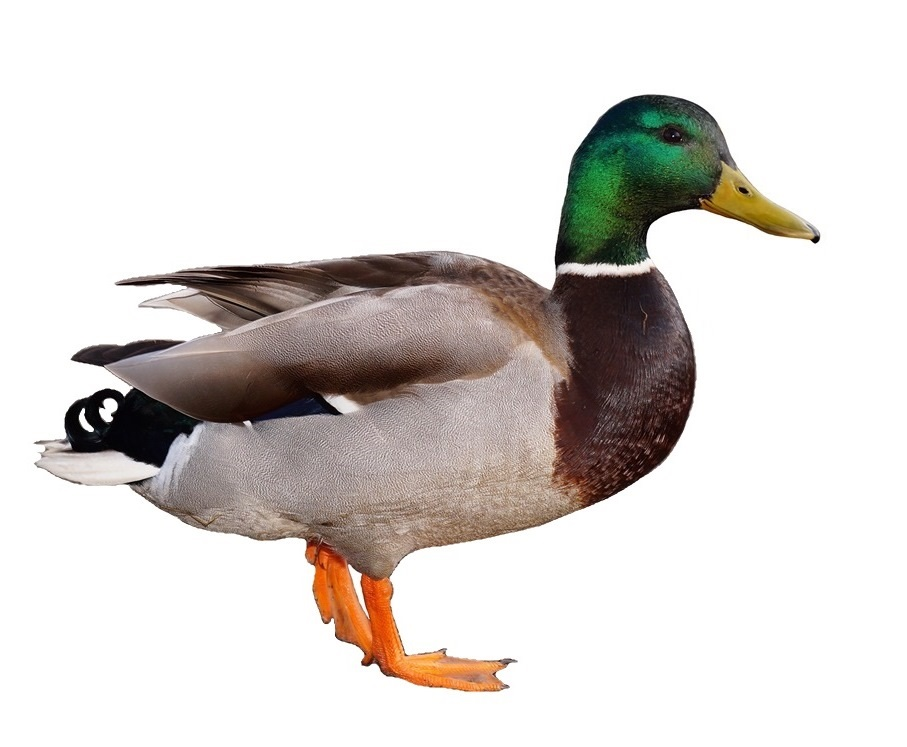
\includegraphics[width=\textwidth]{./figures/duck.jpg}
      \caption{just a duck}
      \label{fig:duck}
    \end{minipage}
%    \hfill
%    \begin{minipage}[c]{0.49\linewidth}
%      \includegraphics[width=\textwidth]{./figures/name of figures.jpg}
%      \caption{}
%      \label{fig:}
%    \end{minipage}
%  \end{center}
%\end{figure}

SORA 2.0 was a continuation of SORA~\cite{SORA} but this time seeking to . . .
Did we complete our objectives?  If yes, what were they again (insert here briefly).  
The main goals for SORA were to once again collect extremophile organisms that reside in the upper atmosphere, study the effects of surrounding radiation on these organisms in the stratosphere and gather data pertaining to the environmental conditions in which these organisms reside~\cite{SORA}.  
SORA 2.0 Objectives here.\\
{\bf Primary Objectives:}
	\begin{enumerate}
	\item Using a refined astrobiology system, attempt to capture bacteria in the upper atmosphere at approximately \SIrange{30}{41}{\kilo\meter} of altitude.
%	\item Study incoming radiation and monitor the surrounding environment using a MiniPIX system with a Boron loaded scintillator.
%	\item Insert more here
	\end{enumerate}
{\bf Secondary Objectives:}
	\begin{enumerate}
	\item Testing the astrobiology hardware in flight and the methodology for collection of microbes in extreme environments at high-altitude.
%	\item Blah
	\end{enumerate}

Past scientifict questions:
 Are extremophiles present in the upper atmosphere at altitudes of 36 to 41 km?  If extremophiles are captured, can the SORA payload clean box container prevent sample contamination? Finally, can we collect data accurately enough to effectively study the effects of environmental radiation on extremophile organisms and spores.
 
 New scientific questions for SORA 2.0:
(Insert here)

\subsection{Hypothesis and Objectives}
\label{subsec:Hypothesis and Objectives}
\begin{enumerate}
%These are from the past year, but they have changed.  Look at the provisional application as well.
%\item Based on the collection results from previous HASP payloads we predict the concentration of cells at an altitude of 36 km will be less than 1000 cells per liter \citep{LSU}.
%	\begin{enumerate}
%	\item Objective: Sample a minimum volumetric amount of air at target altitude for the duration of the float phase (approximately 15 to 18 hours).
%	\item Status: This objective was completed in flight, with successful operation of the sampling pump for the duration of the flight, operating at a confirmed current which allowed for air flow through the sample cell for the entire float portion of the mission.  As of November 28th, 2017 the RNA sequencing results from the lab analysis arrived with positive results.  The full interpretation of the results is currently underway as seen in Section~\ref{sec:Astrobiology-Results}.
%	\end{enumerate}
%\item Based on control samples and testing before flight, we can compare our final flight results to previous applications.
%	\begin{enumerate}
%	\item Objective: Quantify and characterize any contamination with our laboratory and payload disinfection procedures.
%	\item Objective: Minimize the amount of external contamination before flight with thorough decontamination procedures.
%	\item Status: Study is currently underway based on the external lab analysis results which returned RNA sequencing for the collected sample, as well as the control sample.
%	\end{enumerate}
%\item Using SolidWorks 3D CAD design software~\cite{Solidworks} and COMSOL Multiphysics Simulation software~\cite{COMSOL}, we can predict what kind of conditions and forces our container will experience.
%	\begin{enumerate}
%	\item Objective: Using results from simulations and real world tests, adapt a structure and a container to ensure the final results are reliable.
%	\item Status: Incomplete - no simulation results.  Main issue was not having enough time to complete in-depth simulations and actual experimental testing proved more reliable.
%	\end{enumerate}
%\item Based on measured results of dosage rates, the higher exposure to radiation may change the organism's cellular make-up.
%	\begin{enumerate}
%	\item Objective: Quantify the intensity and exposure to UV and cosmic radiation over the duration of the flight.
%	\item Objective: After capturing samples, analyze data and compare biological effects to similar genotypes found on Earth's surface.
%	\item Status: After consultation with biologists at University of Houston (UH), we chose to send the sample for sequencing to see if we captured anything, thus making it hard to compare directly the differences between anything found on Earth and in the atmosphere.  Another mission is necessary to fully complete this objective, but positive results from this mission show the possibilities for a follow-up mission.
%	\end{enumerate}
%\end{enumerate}